% !TeX root = 00Book.tex
\subsection{May: Increase to Four Colonies}

The colonies will probably be in able to make queens in May.
This provides an opportunity to raise two new queens.
The intention is to 
begin the month with two colonies on 18 frames each (9F x 9F)
and 
end the month (or June) with four colonies.  
Two new colonies on 11 frames each (11F)
and 
the two original colonies on 5 or more frames each.\par

\begin{apiary}{Begin with two colonies (and two empty hives)}
    \path (0,0) pic{stand};
    
    \path (4,6) pic{roof};
    \path (4,4) pic{brood=9F};
    \path (4,2) pic{brood=9F};
    \path (4,0) pic{stand};
    
    \path (8,4) pic{roof};
    \path (8,2) pic{brood=2D};
    \path (8,0) pic{stand};

    \path (16,0) pic{stand};
    
    \path (20,6) pic{roof};
    \path (20,4) pic{brood=9F};
    \path (20,2) pic{brood=9F};
    \path (20,0) pic{stand};
    
    \path (24,4) pic{roof};
    \path (24,2) pic{brood=2D};
    \path (24,0) pic{stand};
\end{apiary}

Beside each of the colonies is an empty hive containing two dummy boards.
When a new queen is being raised, the old queen will be removed to the empty hive
and
a new queen will be raised in the original hive.
There is an empty hive stand to the other side of each colony
to allow flying bees to be bled off from the old queen's colony
by swapping the hive to the other side of the new queen.

\subsubsection{Inspect for Queen Raising}

The goal of the inspection is to determine if the colony is considering reproducing,
(not necessarily that full scale swarm preparations are being made).
So we are looking for queen cells with eggs or grubs.

\begin{figure}[H]
\centering
\begin{tikzpicture}
    \color{white}
    \draw (0, 0) node {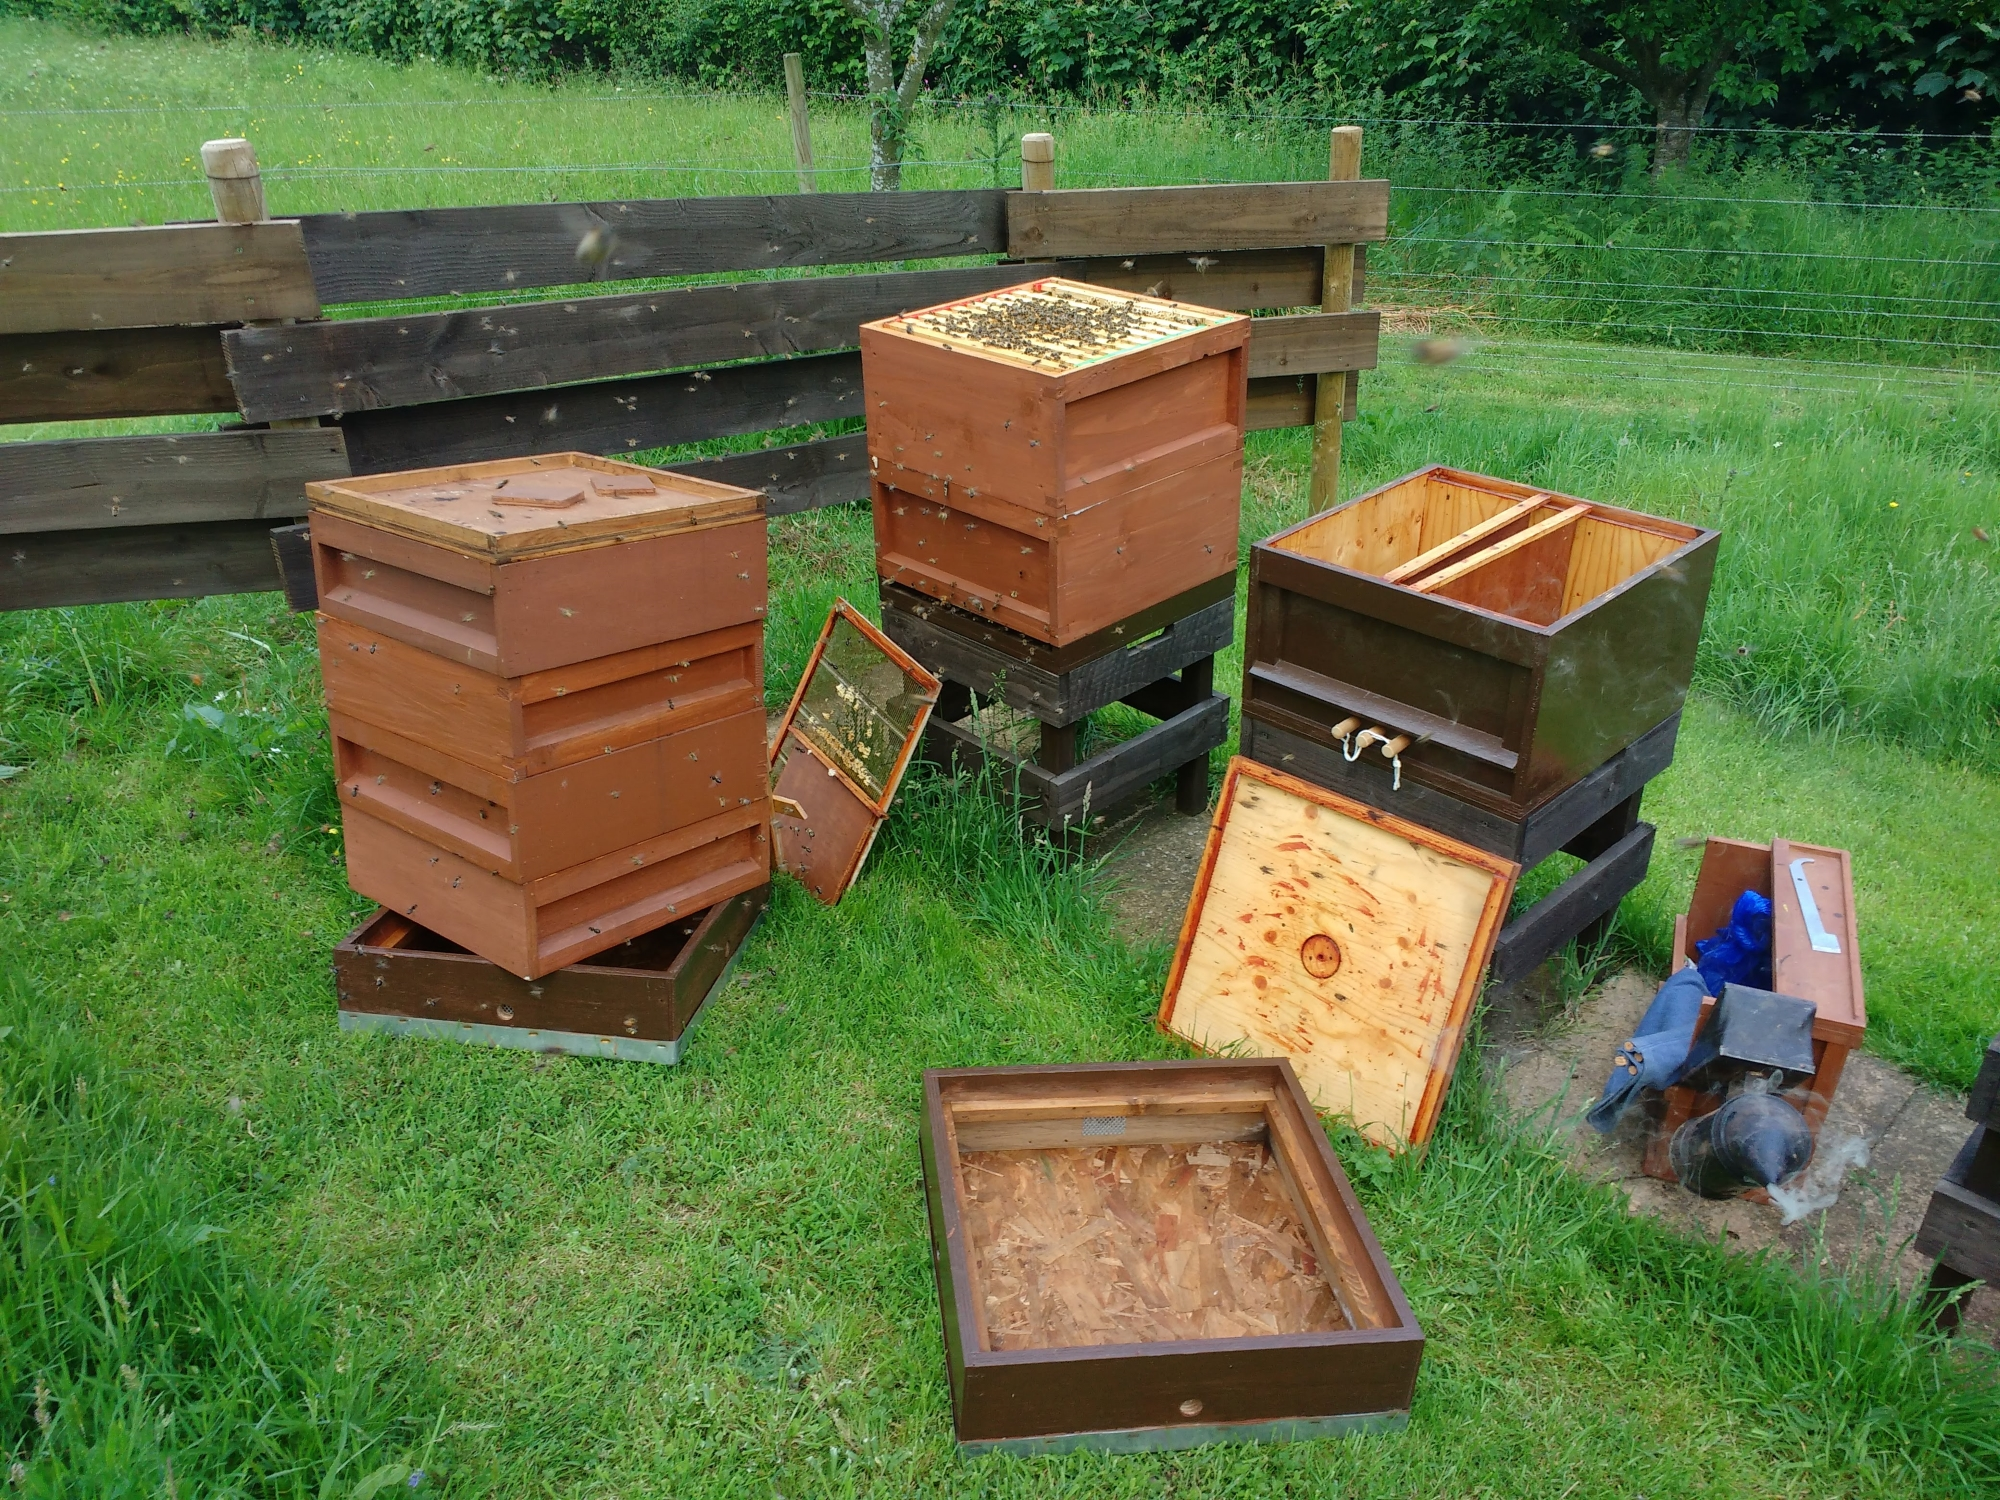
\includegraphics[width=0.9\textwidth]{../assets/05MayInspection.jpg}};
    \draw (0, 2) node {Brood Boxes};
    \draw (-3, 0) node {Supers};
    \draw (3, 0.5) node {Spare Brood Box};
\end{tikzpicture}
\caption{Inspect with supers in front of brood, spare brood box to one side}%
\end{figure}

\begin{description}
  \item [Inspect on a 5 to 6 day interval] to give a margin for error.
    From egg to sealed queen cell takes 8 days, so it is possible to inspect on an 8 day interval and many beekeepers use a 7 day interval.
    However, planned inspections can get delayed, maybe rushed or less than through.
    Reducing the inspection interval to 5 to 6 days gives a greater latitude for errors
    in the event that inspections are delayed by weather or unforeseen circumstances.
  \item [If you see the queen remove that frame] to the spare brood box even if no swarm preparations are apparent.
    Swarm preparations may not be apparent until later in the inspection.
    Putting the queen aside on a single frame in separate box ensures that she available should it be necessary to split the colony.
    If no swarm preparations are apparent the frame with the queen on can be replaced at the end of the inspection.
\end{description}

\subsubsection{Raise a New Queen}

History as a guide to tell you when this might happen.
If you see queen cells with eggs,
then you are good to go.
We are not trying to head off a swarm,
but to breed another queen.

\begin{description}
  \item[Remove queen] If you see queen cells with eggs, remove the queen to one side.
    Re-stack the brood boxes.
    Shake in two frames of bees.
    If there are any sealed queen cells, cull them so that none of the remaining queens will emerge during the next week.
  \item[Cull queen cells] 1 week later cull all cells but one.
    There are probably two because you might have missed one, so there is no need to deliberately leave two.
    Choose a good looking one,
    that doesn't look like it will get damaged by your interference.
  \item[Check for laying] 6 weeks after the queen was removed check for eggs.
    If no eggs add a frame of eggs from the original queen
    and start again. 
\end{description}

Take out the queen to one side along with 7 of the least brood laden frames.  
Add 4 new frames.
Put in a brood box with two dummy boards.
We want the brood to hatch in the production hive.
The queen to one side will be the feeder hive.

The other 11 frames with the queenless hive

\subsubsection*{Step 1: Remove queen}

As soon as occupied queen cells are discovered (eggs or grubs)

Not trying to work out if they are going to swarm.

\begin{description}
  \item[Find queen and remove her], on a frame of (mostly) sealed brood + bees. Remove any queen cells from this frame after checking that there are others in the hive.
  If you can't find her  then guess, she is probably in the middle of the brood nest.
  Then close up the hives and listen.  The noisiest hive is probably queenless.
  Wait and come back in 3 days and look for eggs.
  Put old queen on a stand right beside the stand with the new queen.
  So if there is a problem the two colonies can be united.
  \item[Queen excluder underneath] to prevent swarming (remove after a week)
  \item[Add four other frames] the ones bearing the least brood so the queen has space to lay.
  These will also be the frames with the most stores which could be useful since most of the flying bees will be lost.
  \item[Remove all queen cells] sealed or otherwise.  There shouldn't be any but sometimes you are late and there are sealed cells.
  \item[Shake in three frames of house bees] because most of the flying bees will be lost and these can be promoted to 
  \item[Add three new brood frames] bringing it up to eight frames.  The winter configuration is 8 on 8.
  
  
Put frame + queen in nucleus.
Add a second frame of mostly sealed brood, if wished + a frame of food + another l or 2
frames of comb (preferably) or foundation.
Shake in sufficient young worker bees to ensure that there are enough to cover the brood.
Close up the nucleus. Put green grass in the entrance if it is to remain in the same apiary.
Check through the parent colony.  Mark frames containing 2 or 3 good, unsealed, queen cells with a drawing pin.
Close up the frames in the brood box and till the remaining space with frames of comb or foundation.
  Remove any sealed queen cells (Although, to use this method, the old queen must still be present so there should not be any.)
  \item[Add 4 new frames and feed] 1:2 syrup to draw out the frames
\end{description}

\subsubsection*{Step 2: Remove the Queen Excluder}

After 3 days remove the queen excluder from underneath the original queen,
since the chance of swarming should be reduced now.

\subsubsection*{Step 3: Cull queen cells}

At 7 days after the queen was removed.
There are now no eggs or grubs that can be made into a queen, 
so if the queen cells are culled no more can be created.
Only do this once to minimize disturbance,
if you do it too early they will just make more cells and you will have to do it again.

\begin{description}
  \item[Remove any emergency queen cells] Be meticulous.  Go through it twice.  Brush and smoke, don't shake.
  Go through parent colony and remove any emergency queen cells.
  \item[Keep one (only one) queen cell]
  Select l of the cells previously marked and remove the others.
  Some authorities suggest leaving two, incase one is a dud.
  More than likely you will get a swarm.
  In the event that the one left is a dud the old queen is still available and laying to provide eggs for an emergency queens,
  or to unite back with the colony.
  \item[Add four frames for old queen] The old colony should be building up, add 4 more frames and remove the dummy boards to bring it up to 11 frames.
  \item[Move the old queens colony] to the other side to bleed off bees into the new queens colony.
  \item[Leave for five weeks] looking isn't informative, adding eggs will cause a reset and promote further swarming.
  Don't wait long enough and you might miss the new queen, wait too long and there is a chance of laying worker.
  Five weeks is enough to allow the new queen to come into lay.  Longer than this typically ends with a laying worker.
  But is it a compromise.
\end{description}

Advantages of the method
colony remains strong throughout.
Old queen is kept safe and is available if the new queen does not succeed.
The old queen in the nucleus quickly comes back into lay and her brood can be put back into the parent colony.
The method involves minimum time and lifting.
The nucleus is available to use for other procedures later, or can be united back to the original colony.

\subsubsection*{Step 4: Be Ready for Swarms After Culling}

In the subsequent week be alert for swarms,
If you may have missed a queen cell there are a lot of young bees
so any new queen is like to swarm rather than stay and fight it out.

\subsubsection*{Step 5: Check the Original Queen for Excess Numbers}

Continue inspecting the original queen once a week.
The original queen which was moved to one side may expand quite quickly.
If it does bleed off the flying bees by moving it to the other side of the colony with the queen cells.
This ensures that the original queen is less likely to swarm,
and the the colony with the queen cells has excess flying bees to collect honey.

\subsubsection*{Step 6: Check for a Laying Queen}

At 42 days after the queen was removed
(35 days after the queen cells were culled)
check for a laying queen.

\begin{description}
  \item [If there are is a good brood pattern] look for the new queen and mark her.
  \item [If there are eggs but undeveloped brood] you don't know if it is a good queen or a drone layer.
    Wait for 3 days then recheck, drone laying brood will be obvious at this stage but not over developed.
  \item [If there is drone brood] then there is a drone laying queen or a laying worker.
    Either way take the colony and shake all the bees off the brood frames.
    The flying bees will return to the same location and join the original colony which is to one side.
    Add the brood frames from the failed colony to the original colony to provide space for the flying bees.
  \item [If there is no sign of eggs or brood] then they state of the colony isn't certain.
    Assume that the queen is or will become a drone layer and shake out as above.
    Favouring shaking out rather than uniting because you can't tell if there is a queen or not,
    in which case assume she is present and drone laying.
    At this time point I have never seen a queen not become drone laying,
    so there is little risk of loss.
\end{description}

Shaking out the colony is favoured over uniting with newspaper,
because it ensures that any (bad) queen or laying workers are lost.
Most of the bees should be flying bees at this point,
so there will be only a minimal loss of population.
